\let\negmedspace\undefined
\let\negthickspace\undefined
\documentclass[journal]{IEEEtran}
\usepackage[a5paper, margin=10mm, onecolumn]{geometry}
%\usepackage{lmodern} % Ensure lmodern is loaded for pdflatex
\usepackage{tfrupee} % Include tfrupee package

\setlength{\headheight}{1cm} % Set the height of the header box
\setlength{\headsep}{0mm}     % Set the distance between the header box and the top of the text

\usepackage{gvv-book}
%\usepackage{gvv}
\usepackage{cite}
\usepackage{amsmath,amssymb,amsfonts,amsthm}
\usepackage{algorithmic}
\usepackage{graphicx}
\usepackage{textcomp}
\usepackage{xcolor}
\usepackage{txfonts}
\usepackage{listings}
\usepackage{enumitem}
\usepackage{mathtools}
\usepackage{gensymb}
\usepackage{comment}
\usepackage[breaklinks=true]{hyperref}
\usepackage{tkz-euclide} 
\usepackage{listings}
\usepackage{gvv}                                        
\def\inputGnumericTable{}                                 
\usepackage[latin1]{inputenc}                                
\usepackage{color}                                            
\usepackage{array}                                            
\usepackage{longtable}                                       
\usepackage{calc}                                             
\usepackage{multirow}                                         
\usepackage{hhline}                                           
\usepackage{ifthen}                                           
\usepackage{lscape}
\begin{document}

\bibliographystyle{IEEEtran}

\title{7.4.26}
\author{EE25BTECH11019 - Darji Vivek M.}
{\let\newpage\relax\maketitle}

\renewcommand{\thefigure}{\theenumi}
\renewcommand{\thetable}{\theenumi}
\setlength{\intextsep}{10pt}
\numberwithin{figure}{enumi}
\renewcommand{\thetable}{\theenumi}


\textbf{Question:}\\[2pt]
If two distinct chords, drawn from the point $(p,q)$ on the circle 
\[
x^2 + y^2 = px + qy
\]
(where $pq \ne 0$) are bisected by the $X$-axis, then which of the following is true?
\begin{multicols}{4}
\begin{enumerate}
    \item $p^2 = q^2$
    \item $p^2 = 8q^2$
    \item $p^2 < 8q^2$
    \item $p^2 > 8q^2$
\end{enumerate}
\end{multicols}

\solution \\
Let
\begin{equation}
\vec{P}=\myvec{p\\[2pt] q},\qquad \vec{c}=\frac{1}{2}\vec{P},\qquad r=\frac{1}{2}\sqrt{\vec{P}^\top\vec{P}}.
\end{equation}
(So the circle in translated form is \(\norm{\vec{x}-\vec{c}}=r\).)\\
Let the midpoint of a chord through \(\vec{P}\) lying on the \(x\)-axis be
\begin{equation}
\vec{M}=\myvec{h\\[2pt]0},
\end{equation}
and the other end of the chord be
\begin{equation}
\vec{B}=2\vec{M}-\vec{P}.
\end{equation}
Since \(\vec{B}\) lies on the circle,
\begin{equation}
\brak{\vec{B}-\vec{c}}^\top\brak{\vec{B}-\vec{c}}=r^2.
\end{equation}
Substitute \(\vec{B}=2\vec{M}-\vec{P}\) and \(\vec{c}=\frac12\vec{P}\):
\begin{equation}
\brak{2\vec{M}-\frac{3}{2}\vec{P}}^\top\brak{2\vec{M}-\frac{3}{2}\vec{P}}=\frac{1}{4}\vec{P}^\top\vec{P}.
\end{equation}
Expand and simplify:
\begin{align}
4\vec{M}^\top\vec{M}-6\vec{M}^\top\vec{P}+\frac{9}{4}\vec{P}^\top\vec{P}
&= \frac{1}{4}\vec{P}^\top\vec{P} \\[2pt]
4\vec{M}^\top\vec{M}-6\vec{M}^\top\vec{P}+2\vec{P}^\top\vec{P} &= 0.
\end{align}
With \(\vec{M}=\myvec{h\\[2pt]0}\) we have \(\vec{M}^\top\vec{M}=h^2\) and \(\vec{M}^\top\vec{P}=ph\). Thus
\[
4h^2-6ph+2\vec{P}^\top\vec{P}=0.
\]
Divide by \(2\):
\[
2h^2-3ph+\vec{P}^\top\vec{P}=0.
\]
This quadratic in \(h\) must have two distinct real roots (two distinct chords), so its discriminant is positive:
\begin{align}
\Delta &= 9p^2 - 8\vec{P}^\top\vec{P} > 0 \\[2pt]
&= 9p^2 - 8(p^2+q^2) > 0 \\[2pt]
\implies p^2 - 8q^2 &> 0.
\end{align}
Hence
\[
\boxed{\,p^2>8q^2\,}
\]
(option (d)).

 \begin{figure}[H]
     \centering
     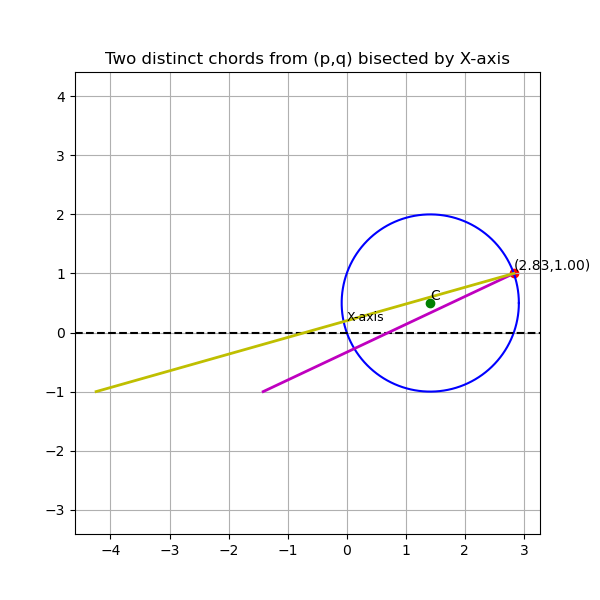
\includegraphics[width=0.8\columnwidth]{figs/14.png}
     \caption{plot if p=2,q=2}
     \label{fig:1}
 \end{figure}
\end{document}